\chapter{The Multilevel Quasidiffusion Method for TRT Problems }
\label{chap-two}
\newcommand{\fd}{\mathcal{D}_T}

In this chapter the discrete forms of the RT, MEB and LOQD equations used in this study are derived. Section \ref{sec:rt_disc} describes the discretization of the multigroup RT equation, section \ref{mloqd_disc} discretizes the multigroup LOQD equations, and section \ref{sec:gloqd_disc} derives the grey LOQD equations from the discretized multigroup LOQD equations. Section \ref{sec:newton} gives discussion of Newton's method used to solve the effective grey problem.

%=================================================================================
% DISCRETE RTE
%=================================================================================
\section{Discretization of the Radiation Transfer Equation} \label{sec:rt_disc}

%=================================================================================
% SN METHOD FOR RTE
%=================================================================================
\subsection{Angular Discretization with Discrete Ordinates} \label{rte_ang_disc}
	The angular dependence of the RT equation is discretized with the method of \textit{discrete-ordinates}. We define a quadrature set
	\begin{equation}
		\crl{ \bOm_m, w_m, m=1,\dots ,N_m }
	\end{equation}
	
	where $\bOm_m$ are discrete directions specified by the angular mesh and $w_m$ are the corresponding quadrature weights such that
	\begin{equation}
		\sum_{m=1}^{N_m}w_m = 4\pi, \quad \sum_{m=1}^{N_m}\bOm_m w_m = 0.
	\end{equation}
	
	The \textit{discrete-ordinates} form of the multigroup RT \eqn{General_RTg_eqn} is
	\begin{equation}
		\frac{1}{c}\dt{\igm\qddepg} + \bOm_m\cdot\grad\igm\qddepg + \kapg\pr{T}\igm\qddepg = \kapg\pr{T}\Bg\pr{T}. \label{Sn_RTE}
	\end{equation}

%=================================================================================
% BACKWARD EULER FOR RTE
%=================================================================================
\subsection{Temporal Discretization with Backward-Euler} \label{rte_time_disc}
	The backward-Euler temporal discretization scheme applied to \eqn{Sn_RTE} is
	\begin{equation}
		\frac{1}{c}\frac{\igmn\rdep - \igmnl\rdep}{\deltn} + \bOm_m\cdot\grad\igmn\rdep + \kapgn\pr{T}\igmn\rdep = \kapgn\pr{T}\Bgn\pr{T} \label{BE_RTE}
	\end{equation}
	
	where $t_n$ is a discrete point in time and $\deltn = t_n - t_{n-1}$. $\igmn\rdep$ is the radiation intensity at time $t_n$, namely, $\igmn\rdep = \igm\pr{\br,t_n}$. Recombining the terms of \eqn{BE_RTE} gives
	\begin{equation}
		\bOm_m\cdot\grad\igmn\rdep + \pr{ \kapgn\pr{T} + \frac{1}{c\deltn} }\igmn\rdep = \kapgn\pr{T}\Bgn\pr{T} + \frac{\igmnl\rdep}{c\deltn} \label{BE_RTE_2}
	\end{equation}
	
	\eqn{BE_RTE_2} takes on the form of a steady state RT equation with a modified source and opacity
	\begin{equation}
		\bOm_m\cdot\grad\igmn\rdep + \modkapgn\pr{T}\igm\rdep = Q_{g,m,n}\pr{T}
	\end{equation}
	
	where the modified source is given as
	\begin{equation}
		Q_{g,m,n}\pr{T} = \kapgn\pr{T}\Bgn\pr{T} + \frac{\igmnl\rdep}{c\deltn} \label{modified_source}
	\end{equation}
	
	and the modified opacity is
	\begin{equation}
		\modkapgn\pr{T} = \kapgn\pr{T} + \frac{1}{c\deltn}. \label{modified_kap}
	\end{equation}

%=================================================================================
% MOC RTE
%=================================================================================
\subsection{Spatial Discretization of the High-Order RT Equation}
	Let us consider Cartesian geometry such that
	\begin{equation}
		\br = \pr{x, y, z}, \quad \grad = \pr{\dx{}, \dy{}, \dz{}}, \label{cartesian}
	\end{equation}
	
	and the solid angle is
	\begin{equation}
		\bOm = \pr{\Omega_x, \Omega_y, \Omega_z}.
	\end{equation}
	
	%Let us introduce the 1D form of the multigroup RT equation \eqref{General_RTg_eqn} by defining the spatial coordinates as Cartesian
	
	
	%The 3D angle $\bOm$ is defined as the product of the azimuthal angle $\gamma$ and the angle $\theta$ such that
	%\begin{equation}
	%	\int_{4\pi} d\Omega = \int_{0}^{\pi} \sin\pr{\theta} d\theta \int_{0}^{2\pi} d\gamma
	%\end{equation}
	
	%One may define the variable $\mu = -\cos\pr{\theta}$ and thus $\dv{\mu}{\theta}= \sin\pr{\theta}$ to give $\bOm$ in terms of the `directional cosine'
	%\begin{equation}
	%	\int_{4\pi} d\Omega = \int_{-1}^{1} d\mu \int_{0}^{2\pi} d\gamma
	%\end{equation}
	
	Figure \ref{fig:solid_angle} depicts the 3D rectangular coordinate system, where $\gamma$ is the angle between the planes formed by the vectors $\bOm$ and $\hat{z}$ and the vectors $\hat{x}$ and $\hat{z}$.
	\begin{figure}[h]
		\centering
		\captionsetup{justification=centering,margin=2cm}
		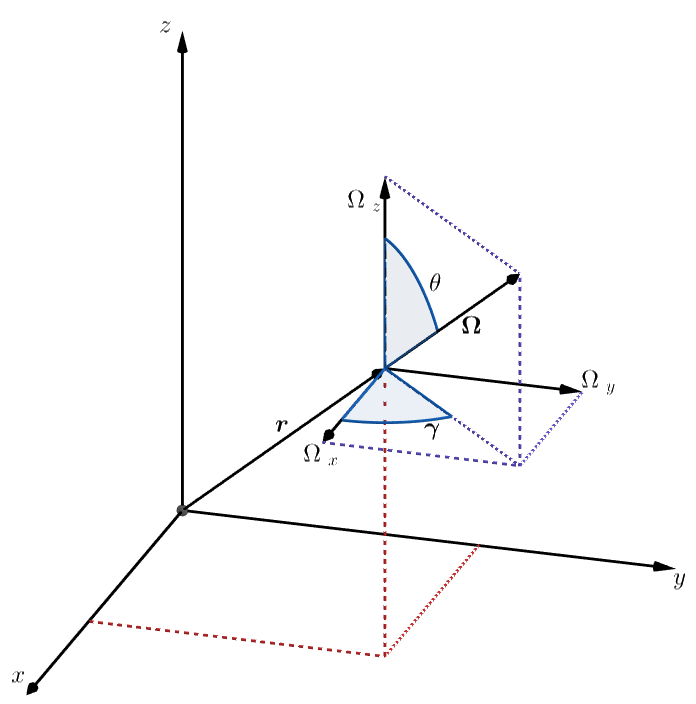
\includegraphics[width=.5\textwidth]{solid_angle2.png} 
		\caption{\label{fig:solid_angle}
			Rectangular Coordinate System}
	\end{figure}

	%From 3D Cartesian geometry, a geometry with no dependence on the $\hat{x}$ and $\hat{y}$ directions, known as 1D slab geometry, can be derived. 
	
	The 3D RT equation \eqref{General_RTg_eqn} can be reduced to 1D slab geometry form where the solution is a function only of the variables $z$ and $\theta$. 1D slab geometry, or plane geometry, is formulated such that the $\hat{x}$ and $\hat{y}$ directions are assumed infinite and material composition does not depend on these directions. Thus the behavior of radiation propagating out in those directions has translational geometry and change is only observed along the $\hat{z}$ axis for different $\pr{\hat{x}, \ \hat{y}}$ planes. The path length $ds$ of propagating radiation can then be written as a function of the distance moved along the $\hat{z}$ axis $(dz)$ and the angle between direction of movement and the $\hat{z}$ axis $\pr{\theta}$
	\begin{equation}
		ds = cos\pr{\theta}dz. \label{ds}
	\end{equation}
	
	\begin{figure}[h]
		\centering
		\captionsetup{justification=centering,margin=2cm}
		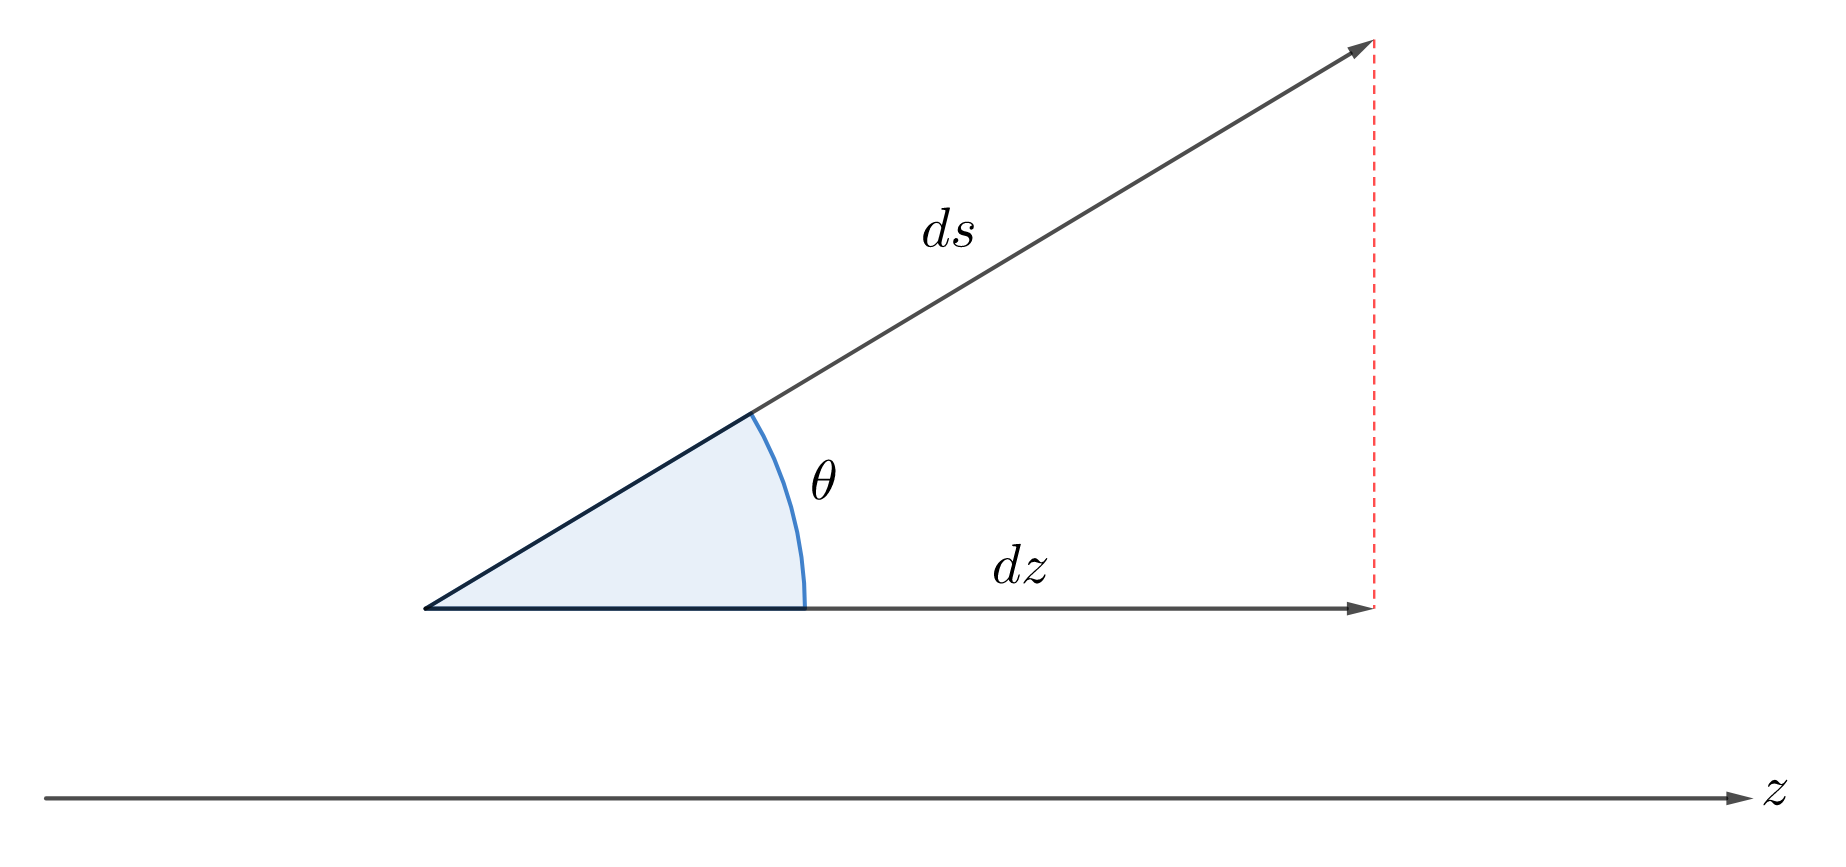
\includegraphics[width=\textwidth]{1dslab.png} 
		\caption{\label{fig:1dslab_geom}
			Path length in 1D slab geometry}
	\end{figure}
	
	Figure \ref{fig:1dslab_geom} depicts the path length described in Eq. \eqref{ds} for 1D slab geometry. The spatial coordinate system \eqref{cartesian} reduces to
	\begin{equation}
		\br = \pr{z}, \quad \grad = \pr{\dz{}}. \label{1d_cartesian}
	\end{equation}
	
	The streaming operator is also reduced by noting $\bOm \cdot \grad \ig = \dv{\ig}{s}$ so that with Eq. \eqref{ds} 
	\begin{equation}
		\bOm \cdot \grad \ig = \dv{\ig}{s} = \dv{\ig}{z}\dv{z}{s} = \dv{\ig}{z}cos\pr{\theta}.
	\end{equation}
	
	The directional cosine is defined as $\mu = cos\pr{\theta}$ so $\bOm \cdot \grad \ig = \mu\cdot\dv{\ig}{z}$. The solution of the RT equation only depends on $z$ and $\mu$ and hence $\ig\pr{\br,\bOm,t} = \ig\pr{z,\mu,t}$. We now integrate the RT equation over $0\leq\gamma\leq 2\pi$ to obtain the 1D slab geometry form of the multigroup RT equation, given by
	\begin{gather}
		\frac{1}{c}\dt{\tilde{I}_g\pr{z,\mu,t}} + \mu\cdot\dx{\tilde{I}_g\pr{z,\mu,t}} + \kapg\pr{T}\tilde{I}_g\pr{z,\mu,t} = 2\pi\kapg\pr{T}\Bg\pr{T}, \label{1D_RTEgz}\\
		0\leq z\leq Z, \quad -1\leq\mu\leq 1, \quad t\geq t_0, \nn
	\end{gather}
	
	where $\tilde{I}_g\pr{z,\mu,t} = 2\pi I_g\pr{z,\mu,t}$ To remain consistent with the usual notation, a notation change is performed such that $\tilde{I}_g\pr{z,\mu,t} \ra I_g\pr{x,\mu,t}$ to rewrite Eq. \eqref{1D_RTEgz} as
	\begin{gather}
		\frac{1}{c}\dt{\ig\pr{x,\mu,t}} + \mu\cdot\dx{\ig\pr{x,\mu,t}} + \kapg\pr{T}\ig\pr{x,\mu,t} = 2\pi\kapg\pr{T}\Bg\pr{T}, \label{1D_RTEg}\\
		0\leq x\leq X, \quad -1\leq\mu\leq 1, \quad t\geq t_0 \nn.
	\end{gather}
	
	Boundary conditions for Eq. \eqref{1D_RTEg} are
	\begin{subequations}
		\begin{align}
			\ig|_{x=0} = \ig^{\text{in},+}\pr{\mu,t}, \quad &\mu>0 \\
			\ig|_{x=X} = \ig^{\text{in},-}\pr{\mu,t}, \quad &\mu<0.
		\end{align}
	\end{subequations}
	
	To discretize the 1D slab geometry RT equation in angle with \textit{discrete-ordinates} a new quadrature set is constructed for $\mu$
	\begin{equation}
		\crl{ \mu_m,\ w_m,\ m=1,\dots ,N_m }
	\end{equation}
	
	where $\mu_m$ are discrete directional cosines specified by the angular mesh and $w_m$ are the corresponding quadrature weights such that
	\begin{equation}
		\sum_{m=1}^{N_m}w_m = 2, \quad \sum_{m=1}^{N_m}\mu_m w_m = 0.
	\end{equation}
	
	Discretizing \eqn{1D_RTEg} with discrete ordinates over angle (Sec. \ref{rte_ang_disc}) and backward-Euler over time (Sec. \ref{rte_time_disc}) yields
	\begin{equation}
		\mu_m\frac{d\igmn\pr{x}}{dx} + \pr{ \kapgn\pr{T} + \frac{1}{c\deltn} }\igmn\pr{x} = \kapgn\pr{T}\Bgn\pr{T} + \frac{\igmnl\pr{x}}{c\deltn}. \label{1D_RTEg_disc}
	\end{equation}	
	
	To discretize the 1D slab geometry RT equation in space a spatial mesh is introduced	
	\begin{equation}
		\crl{ x_{i+\frac{1}{2}}, \quad i=1,\dots ,N_i, \quad 0=x_{\frac{1}{2}}<\dots<x_{i+\frac{1}{2}}<\dots<x_{N_i+\frac{1}{2}}=X }, \label{xmesh}
	\end{equation}
	
	shown in Figure \ref{fig:1Dmesh}. The length of each cell is $\delxi = x_{i+\frac{1}{2}} - x_{i-\frac{1}{2}}$. Cell centers are located at positions $x_i = x_{i-\frac{1}{2}} + \frac{1}{2}\delxi$.
	\begin{figure}[h]
		\centering
		\captionsetup{justification=centering,margin=2cm}
		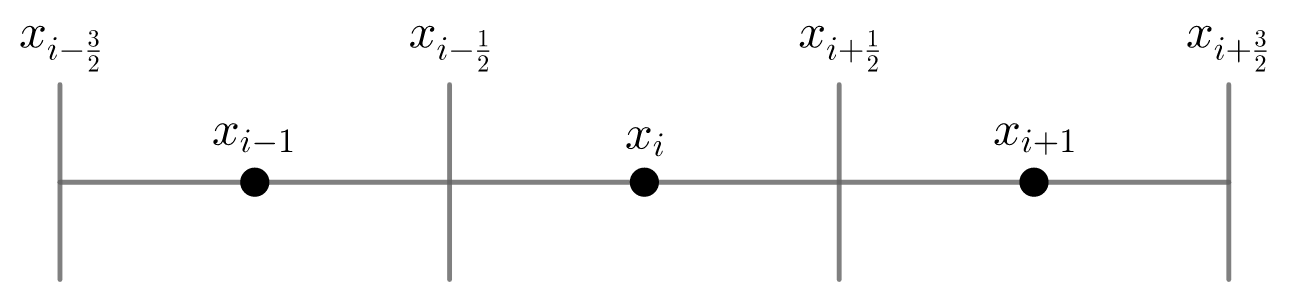
\includegraphics[width=.5\textwidth]{1Dmesh.png}
		\caption{\label{fig:1Dmesh}
			1D spatial mesh grid}
	\end{figure}
	
	%This mesh is designed with the physics of the radiative transfer problem in mind, such that $x_{i+\frac{1}{2}}$ is the right `cell face' and $x_{i-\frac{1}{2}}$ is the left `cell face' of cell $i$. This is done so that the radiation intensity at each `cell face' may be calculated, along with the average intensity per cell. The cell edge radiation intensity is defined as
	
	The discretization scheme formulated on this mesh is known as step characteristics, which follows from the method of characteristics and is defined for cell-average and cell-edge values of the radiation intensity. The radiation intensity at time $t_n$, direction $\mu_m$ and position $x_{i+\frac{1}{2}}$ is written as $\igmirn$. The step characteristics discretization scheme for \eqn{1D_RTEg_disc} for cell-edge radiation intensities is
	\begin{subequations}
		\begin{align}
			&\igmiln = \igmirn e^{-\tau_{g,m,i}} + \frac{Q_{g,m,i,n}}{\modkapgin}\pr{1 - e^{-\tau_{g,m,i}}}, \quad \mu_m > 0\\
			&\igmirn = \igmiln e^{-\tau_{g,m,i}} + \frac{Q_{g,m,i,n}}{\modkapgin}\pr{1 - e^{-\tau_{g,m,i}}}, \quad \mu_m < 0
		\end{align}
		\label{step_edges}
	\end{subequations}
	
	and the equation for cell-average radiation intensities is
	\begin{equation}
		\igmin = \alpha_{g,m,i}\igmiln + \pr{1-\alpha_{g,m,i}}\igmirn, \label{step_avgs}
	\end{equation}
	
	where the source $Q_{g,m,i,n}$ and modified opacity $\modkapgin$ are cell-average quantities given by Eqs. \eqref{modified_source} and \eqref{modified_kap}, respectively. $\tau_{g,m,i}$ is
	\begin{equation}
		\tau_{g,m,i} = \frac{\modkapgin\delxi}{\abs{\mu_m}},
	\end{equation}
	
	and $\alpha_{g,m,i}$ is
	\begin{equation}
		\alpha_{g,m,i} = \left\{ \begin{array}{ll}
			\frac{1}{\tau_{g,m,i}} - \frac{e^{-\tau_{g,m,i}}}{1-e^{-\tau_{g,m,i}}}, & \mu_m>0\\
			-\frac{1}{\tau_{g,m,i}} + \frac{1}{1-e^{-\tau_{g,m,i}}}, & \mu_m<0.
		\end{array} \right.
	\end{equation}
	
%=================================================================================
% DISCRETE MLOQD
%=================================================================================
\section{Discretization of the MLOQD Equations} \label{mloqd_disc}

%=================================================================================
% BACKWARD EULER FOR MLOQD
%=================================================================================
\iffalse
\subsection{Temporal Discretization with Backward-Euler Scheme}
	The backward-Euler temporal discretization scheme applied to the MLOQD Eqs. \eqref{mqd_sys} is
	\begin{subequations}
		\begin{gather}
			\frac{\egn\rdep - \egnl\rdep}{\deltn} + \grad\cdot\bFgn\rdep + c\kapgn\pr{T}\egn\rdep = 4\pi\kapgn\pr{T}\Bgn\pr{T} \label{mqd_1_n}\\
			\frac{1}{c}\frac{\bFgn\rdep - \bFgnl\rdep}{\deltn} + c\grad\cdot\pr{\bfgn\rdep\egn\rdep} + \kapgn\pr{T}\bFgn\rdep = 0 \label{mqd_2_n}
		\end{gather}
	\end{subequations}
	
	where $\egn\rdep$, $\bFgn\rdep$ and $\bfgn\rdep$ are the group radiation energy density, flux and QD factors at time $t_n$.	recombining the terms of Eqs. \eqref{mqd_1_n} and \eqref{mqd_2_n}, respectively gives
	\begin{subequations}
		\begin{gather}
			\grad\cdot\bFgn\rdep + c\pr{\kapgn\pr{T} + \frac{1}{c\deltn}}\egn\rdep = 4\pi\kapgn\pr{T}\Bgn\pr{T} + \frac{\egnl\rdep}{\deltn}  \label{mqd_1_recomb}\\
			c\grad\cdot\pr{\bfgn\rdep\egn\rdep} + \pr{\kapgn\pr{T} + \frac{1}{c\deltn}}\bFgn\rdep = \frac{\bFgnl\rdep}{c\deltn} \label{mqd_2_recomb}
		\end{gather}
		\label{mqd_recombs}
	\end{subequations}
	
	and as seen for the radiative transfer equation in Section \ref{rte_time_disc}, Eqs. \eqref{mqd_recombs} take the form of a steady state multigroup LOQD system with a modified source and opacity
	\begin{subequations}
		\begin{gather}
			\grad\cdot\bFgn\rdep + c\modkapgn\pr{T}\egn\rdep = 4\pi\kapgn\pr{T}\Bgn\pr{T} + \frac{\egnl\rdep}{\deltn}  \label{mqd_1_mod}\\
			c\grad\cdot\pr{\bfgn\rdep\egn\rdep} + \modkapgn\pr{T}\bFgn\rdep = \frac{\bFgnl\rdep}{c\deltn} \label{mqd_2_mod}
		\end{gather}
		\label{mqd_mods}
	\end{subequations}
	
	where the modified opacity is given by \eqn{modified_kap}.
\fi
%=================================================================================
% FINITE VOLUME FOR MLOAM
%=================================================================================
%\subsection{1D Finite Volume}
	The MLOQD equations in 1D slab geometry are
	\begin{subequations}
		\begin{gather}
			\dt{\eg\pr{x,t}} + \dx{\Fg\pr{x,t}} + c\kapg\pr{T}\eg\pr{x,t} = 4\pi\kapg\pr{T}\Bg\pr{T}, \label{mqd_1_1d} \\
			\frac{1}{c}\dt{\Fg\pr{x,t}} + c\dx{\pr{\bfg\pr{x,t}\eg\pr{x,t}}} + \kapg\pr{T}\Fg\pr{x,t} = 0, \label{mqd_2_1d}\\
			0\leq x\leq X, \quad t\geq t_0, \quad g=1,\dots,N_g, \nn
		\end{gather}
		\label{1dmloqd}
	\end{subequations}
	
	with boundary conditions
	\begin{subequations}
		\begin{gather}
			\Fg\pr{0,t} = cC_g^0\pr{t}\pr{\eg\pr{0,t} - E_g^{\text{in},+}\pr{t}} + \Fg^{\text{in},+}\pr{t}, \quad \mu>0\\
			\Fg\pr{X,t} = cC_g^X\pr{t}\pr{\eg\pr{X,t} - E_g^{\text{in},-}\pr{t}} + \Fg^{\text{in},-}\pr{t}, \quad \mu<0
		\end{gather}
	\end{subequations}
	
	where the group boundary factors are
	\begin{align}
		\cgl = \left. \frac{\int_{-1}^{0} \mu\ig d\mu }{\int_{-1}^{0} \ig d\mu} \right|_{x=0}, \quad \cgr = \left. \frac{\int_{0}^{1} \mu\ig d\mu }{\int_{0}^{1} \ig d\mu} \right|_{x=0}.
	\end{align}
	
	The backward-Euler temporal discretization scheme applied to Eqs. \eqref{1dmloqd} is
	\begin{subequations}
		\begin{gather}
			\dx{\Fgn\pr{x}} + c\modkapgn\egn\pr{x} = 4\pi\kapgn\pr{T}\Bgn + \frac{\egnl\pr{x}}{\deltn},  \label{mqd_1_1dn}\\
			c\dx{\pr{\fgn\pr{x}\egn\pr{x}}} + \modkapgn\Fgn\pr{x} = \frac{\Fgnl\pr{x}}{c\deltn} \label{mqd_2_1dn},
		\end{gather}
	\end{subequations}
	
	%We consider the spatial mesh \eqref{xmesh} as shown in Figure \ref{fig:1Dmesh} for spatial discretization. The aim of this discretization is to find a system of equations in terms of the `cell-edge' radiation fluxes and `cell-average' radiation energy densities. This is based on the units of each of these quantities, since the radiation flux is the intensity of radiation moving through a plane and the radiation energy density is the intensity of radiation present in a given volume. 
	
	A second-order finite volume scheme is used to disctretize the MLOQD system in space. The radiation energy balance \eqn{mqd_1_1dn} is integrated over the spatial interval of the $i^{th}$ cell $x_{i-\frac{1}{2}}\leq x\leq x_{i+\frac{1}{2}}$ to give
	\begin{equation}
		\Fgirn - \Fgiln + c\delxi\modkapgin\egin = \delxi\pr{4\pi\kapgin\Bgin + \frac{\eginl}{\deltn}}, \label{mqd_1_disc}
	\end{equation}
	
	where $\Fgirn$ is the cell-edge value of the group-wise radiation flux and $\egin$ is the cell-averaged value of the group-wise radiation energy density. The radiation momentum balance \eqn{mqd_2_1dn} is integrated over the the $i^{th}$ cell's left half $x_{i-\frac{1}{2}}\leq x\leq x_{i}$ and over its right half $x_{i}\leq x\leq x_{i+\frac{1}{2}}$. This gives two discretized equations
	\begin{gather}
		c\pr{\fgin\egin - \fgiln\egiln} + \frac{\delxi}{2}\modkapgin\Fgiln = \frac{\delxi}{2}\frac{\Fgilnl}{c\deltn}, \label{mloqd_disc_left}\\
		c\pr{\fgirn\egirn - \fgin\egin} + \frac{\delxi}{2}\modkapgin\Fgirn = \frac{\delxi}{2}\frac{\Fgirnl}{c\deltn} \label{mloqd_disc_right}.
	\end{gather}
	
	To eliminate the cell-edge radiation energy density $\egirn$, \eqn{mloqd_disc_left} is found for the $i+1$ cell and combined with \eqn{mloqd_disc_right} to obtain
	\begin{equation}
		c\pr{\fgirrn\egirrn - \fgin\egin} + \delxir\modkapgirn\Fgirn = \delxir\frac{\Fgirnl}{c\deltn}, \label{mqd_2_disc}
	\end{equation}
	
	where
	\begin{equation}
		\delxir = \frac{\delxi + \delxirr}{2},
	\end{equation}
	
	with $\Delta x_0=0$, $\Delta x_{I+1}=0$, and the cell-edge opacity is
	\begin{equation}
		\kapgirn = \frac{\delxi\kapgin+\delxirr\kapgirrn}{\delxi+\delxirr}, \ \ \modkapgirn = \frac{\delxi\modkapgin+\delxirr\modkapgirrn}{\delxi+\delxirr}.
	\end{equation}
	
	The discrete MLOQD system is thus
	\begin{subequations}
		\begin{gather}
			\Fgirn - \Fgiln + c\delxi\modkapgin\egin = \delxi\pr{4\pi\kapgin\Bgin + \frac{\eginl}{\deltn}} \label{mqd_1_disc_2},\\
			c\pr{\fgirrn\egirrn - \fgin\egin} + \delxir\modkapgirn\Fgirn = \delxir\frac{\Fgirnl}{c\deltn} \label{mqd_2_disc_2}.
		\end{gather}
		\label{mqd_sys_disc}
	\end{subequations}
	
	The discretized MLOQD Eqs. \eqref{mqd_sys_disc} give a system of equations for the group radiation flux and energy density. Eqs. \eqref{mqd_sys_disc} can be manipulated to eliminate the group radiation flux and create a smaller linear system, demonstrated for the GLOQD system in Sec. (\ref{sec:gloqd_disc}).
	
%=================================================================================
% DISCRETE GLOQD
%=================================================================================
\section{Discretization of the GLOQD and MEB Equations} \label{sec:gloqd_disc}

%=================================================================================
% BACKWARD EULER FOR GLOQD
%=================================================================================
%\subsection{Discretization of the GLOQD and MEB Equations} \label{gloqd_disc}
	To maintain algebraic consistency between the discretization of the MLOQD equations and the GLOQD equations, the discrete GLOQD equations are derived from the discrete MLOQD Eqs. \eqref{mqd_sys_disc} by summing them over group. The discrete GLOQD equations are thus
	\begin{subequations}
	\begin{equation}
		\Fbirn - \Fbiln + c\delxi\modkapebin\ebin = \delxi\pr{c\kapbbin\ar T^4_{i,n} + \frac{\ebinl}{\deltn}}, \label{gqd_1_disc}
	\end{equation}
	\vspace*{-1cm}
	\begin{multline}
		c\pr{\fbirrn+\etairnp}\ebirrn - c\pr{\fbin+\etairnm}\ebin \\+ \delxir\modkaprbirn\Fbirn = \delxir\frac{\Fbirnl}{c\deltn}. \label{gqd_2_disc}
	\end{multline}
	\label{gqd_sys_disc}
	\end{subequations}
	
	where the total cell-averaged radiation energy density is
	\begin{equation}
		\ebin = \sum_{g=1}^{N_g}\egin,
	\end{equation}
	
	and the total cell face averaged radiation flux is
	\begin{equation}
		\Fbirn = \sum_{g=1}^{N_g}\Fgirn.
	\end{equation}
	
	The group QD factor in each cell is averaged with the cell-averaged group energy density to form the cell-averaged grey QD factor
	\begin{equation}
		\fbin = \frac{\sum_{g=1}^{N_g} \fgin\egin}{\sum_{g=1}^{N_g} \egin}.
	\end{equation}
	
	The two modified grey opacities are
	\begin{gather}
		\modkapebin = \kapebin + \frac{1}{c\deltn}, \label{modkapE} \\
		\modkaprbirn = \kaprbirn + \frac{1}{c\deltn},
	\end{gather}
	
	and the three distinct grey opacities in each cell or cell face are
	\begin{gather}
		\kapebin = \frac{ \sum_{g=1}^{N_g}\kapgin\egin }{ \sum_{g=1}^{N_g}\egin }, \\[5pt]
		\kapbbin = \frac{ \sum_{g=1}^{N_g}\kapgin\Bgin }{ \sum_{g=1}^{N_g}\Bgin }, \\[5pt]
		\kaprbirn = \frac{ \sum_{g=1}^{N_g}\kapgirn\abs{\Fgirn} }{ \sum_{g=1}^{N_g}\abs{\Fgirn} }.
	\end{gather}
	
	The compensation term takes the form
	\begin{subequations}
		\begin{align}
			&\etairn = \sum_{g=1}^{N_g} \brk{\pr{\kapgirn - \kaprbirn}\Fgirn},\\
			&\etairnp = \left\{ \begin{array}{ll}
							\frac{\etairn}{\sum_{g=1}^{N_g} \egirrn}, & \etairn>0,\\
							0, & \etairn<0,
						\end{array} \right.\\
			&\etairnm = \left\{ \begin{array}{ll}
							0, & \etairn>0,\\
							\frac{-\etairn}{\sum_{g=1}^{N_g} \egin}, & \etairn<0.
						\end{array} \right.
		\end{align}
	\end{subequations}
	
	The terms $\eta^{\pm}$ are defined as such so that the coefficient multiplying the total radiation energy density in the radiation momentum balance Eq. \eqref{gqd_2_disc} does not become negative. The discretized GLOQD Eqs. \eqref{gqd_sys_disc} give a system of equations for the total radiation flux and energy density. %One may eliminate the total radiation flux from \eqn{gqd_1_disc} by using \eqn{gqd_2_disc} to substitute and create a smaller linear system to solve for only the cell-average total radiation energy density.
	
	\ind Now considering the MEB equation \eqref{Energy_Balance_gr}, the 1D slab geometry form is
	\begin{equation}
		\dt{\varepsilon\pr{T}} = c\kapeb\pr{T}\eb\pr{x,t} - c\kapbb\pr{T}\ar T^4. \label{Energy_Balance_gr2}
	\end{equation}
	
	%One can make the assumption that the material energy density $\varepsilon\pr{T}$ is simply the specific heat of the material $\cv$ times the material temperature $T$
	%\begin{equation}
	%	\varepsilon\pr{T} = \cv T,
	%\end{equation}
	
	%which gives a new form of the MEB equation
	%\begin{equation}
	%	\cv\dt{T} = c\kapeb\pr{T}\eb\pr{x,t} - c\kapbb\pr{T}\ar T^4. \label{Energy_Balance_gr3}
	%\end{equation}
	
	\eqn{Energy_Balance_gr2} then takes on the discrete form
	\begin{equation}
	%	\cv\frac{\tin - \tinl}{\delt} = c\kapebin\ebin - c\ar\kapbbin\tin^4. \label{ebdisc}
		\frac{\varepsilon_{i,n}\pr{T} - \varepsilon_{i,n-1}\pr{T}}{\delt_n} = c\kapebin\ebin - c\ar\kapbbin\tin^4. \label{ebdisc}
	\end{equation}
	
	The GLOQD equations \eqref{gqd_sys_disc} share a source term with the MEB Eq. \eqref{ebdisc}
	\begin{equation}
		\qbin = c\ar\kapbbin\tin^4. \label{grsource}
	\end{equation}
	
%\subsection{Removing the Radiation Flux from the Effective Grey Problem \label{Fremove}}
	A reduced system is derived from the GLOQD \eqref{gqd_sys_disc} and MEB \eqref{ebdisc} equations by eliminating the total radiation flux. The terms of the grey radiation momentum balance Eq. \eqref{gqd_2_disc} are recombined as
	\begin{equation}
		\Fbirn = \bar{h}_i - \Dirnp\ebirrn + \Dirnm\ebin, \label{Fisolate}
	\end{equation}
	
	where
	\begin{gather}
		\bar{h}_i = \frac{\Fbirnl}{c\delt\kaprbirn+1}, \\
		\Dirnp = \frac{c\fbirrn + \etairnp}{\delxir\modkaprbirn}, \\
		\Dirnm = \frac{c\fbin + \etairnm}{\delxir\modkaprbirn}.
	\end{gather}
	
	%$\Fbirn$ and $\Fbiln$ in Eq. \eqref{gqd_1_disc} are replaced with Eq. \eqref{Fisolate} to give
	%\begin{multline}
	%	\pr{- \Dirnp\ebirrn + \Dirnm\ebin} - \pr{- \Dilnp\ebin + \Dilnm\ebilln} + c\delx\modkapebin\ebin \\= \delx\qbin + \frac{\delx\ebinl}{\delt} - \bar{h}_i + \bar{h}_{i-1}.
	%\end{multline}
	
	$\Fbirn$ and $\Fbiln$ in Eq. \eqref{gqd_1_disc} are replaced with Eq. \eqref{Fisolate} to give the discrete system of GLOQD and MEB equations
	\begin{subequations}
		\begin{multline}
			- \Dilnm\ebilln + \pr{\Dirnm + \Dilnp + c\delx\modkapebin}\ebin - \Dirnp\ebirrn \\ = \delx\qbin + P_{i,n-\frac{1}{2}}, \label{gqd_E}
		\end{multline}
		\vspace*{-.5cm}
		\begin{equation}
			\frac{\varepsilon_{i,n} - \varepsilon_{i,n-1}}{\delt_n} = c\kapebin\ebin - \qbin, \label{ebdisc2}
		\end{equation}
		\label{reduced_gr_sys}
	\end{subequations}

	with Eq. \eqref{Fisolate} as an auxiliary used to calculate radiation flux values from the solution of \eqref{reduced_gr_sys} and
	\begin{equation}
		P_{i,n-\frac{1}{2}} = \frac{\delx_i\ebinl}{\delt_n} + \bar{h}_{i-1} - \bar{h}_{i}.
	\end{equation}
	
	
	
%=================================================================================
% 
%=================================================================================
%\section{The QD System}
%	The full system of equations used in the QD method contains the RT, multigroup LOQD and grey LOQD Eqs. \eqref{step_edges}, \eqref{step_avgs}, \eqref{mqd_sys_disc} \& \eqref{gqd_sys_disc}.
	%\begin{subequations}
	%	\begin{gather}
	%		
	%	\end{gather}
	%\end{subequations}

%=================================================================================
% Coupling the Grey low-order and Energy Balance Equations
%=================================================================================
\section{Newton's Method for the GLOQD and MEB Equations} \label{sec:newton}
	Newton's method \cite{kelley-newton} is used to solve the GLOQD and MEB Eqs. \eqref{reduced_gr_sys}. It is an iterative method to find the roots of a given system of nonlinear equations
	\begin{equation}
		\bm{G}\pr{\bx} = 0. \label{Gdef}
	\end{equation}
	
	The system of equations is linearized about some estimate of the solution to obtain
	\begin{equation}
		\bm{G}\pr{\bx^{\pr{s}}} + \bm{G}'\pr{\bx^{\pr{s}}}\pr{\bx-\bx^{\pr{s}}} = 0, \label{linear}
	\end{equation}
	
	where $\bG'$ is the Jacobian of the system, and $\bx^{\pr{s}}$ is the solution of the $s^{\text{th}}$ iterate. Eq. \eqref{linear} is then rewritten as
	\begin{equation}
		\Delta \bx^{\pr{s}} =  - \pr{\bG'\pr{\bx^{\pr{s}}}}^{-1}\bm{G}\pr{\bx^{\pr{s}}},
	\end{equation}
	
	where $\Delta \bx^{\pr{s}} = \bx-\bx^{\pr{s}}$. The solution of the following iterate is defined as
	\begin{equation}
		\bx^{\pr{s+1}} = \bx^{\pr{s}} + \Delta \bx^{\pr{s}},
	\end{equation}
	
	thus
	\begin{equation}
		\bx^{\pr{s+1}} = \bx^{\pr{s}} - \pr{\bG'\pr{\bx^{\pr{s}}}}^{-1}\bm{G}\pr{\bx^{\pr{s}}}.
	\end{equation}
	
	The discretized GLOQD and MEB Eqs. \eqref{reduced_gr_sys} form a system for the total radiation energy density and temperature vectors $\pr{\bE,\bT}$. We define
	\begin{gather}
		\ebinsrv = \ebinsv + \debinsv \label{dele}\\
		\tinsrv = \tinsv + \dtinsv, \label{delt}
	\end{gather}
	
	where $\debinsv$ and $\dtinsv$ are the iterative increments for the radiation energy density and temperature, respectively. The grey functions that depend on temperature are also linearized, namely the opacity $(\kapeb)$, material energy density $(\varepsilon)$ and source term $(\qb)$ to get
	\begin{gather}
		\varepsilon_{i,n}^{\pr{s+1}} = \varepsilon_{i,n}^{\pr{s}} + \frac{d\varepsilon_{i,n}^{\pr{s}}}{dT}\dtinsv,\\
		\qbinsrv = \qbinsv + \frac{d\qbinsv}{dT}\dtinsv, \\
		%\kapebin^{\pr{s+1}} = \kapebin^{\pr{s}} + \dv{\kapebin^{\pr{s}}}{T}\dtinsv,\\
		\kapebin^{\pr{s+1}} = \kapebin^{\pr{s}} + \pr{\fd \kapebin}^{\pr{\ell}}\dtinsv. \label{frechet}
	\end{gather}
	
	The source term and material energy density are known local functions of temperature and thus their derivatives with respect to $T$ can be directly calculated. The opacity $\kapeb$ however, is an averaged quantity over the entire spectrum range. Thus the grey opacity depends not only on the change in the multi-group opacity, but also on the spectrum change and is thus globally dependent on temperature. The Fr\'echet derivative $\pr{\fd \kapebin}^{\pr{\ell}}$ must be approximated to take into account the variation in energy density spectrum. Here $\ell$ denotes the index of the MLOQD iteration. This Fr\'echet derivative is calculated using the value of the grey opacity and temperature at successive MLOQD iterations
	\begin{equation}
		\pr{\fd \kapebin}^{\pr{\ell}} = \frac{\kapebin^{\pr{\ell}} - \kapebin^{\pr{\ell-1}}}{\tin^{\pr{\ell}} - \tin^{\pr{\ell-1}}}, \label{frachet2}
	\end{equation}
	
	The use of Eqs. \eqref{frechet} and \eqref{frachet2} lead to an approximate Jacobian. Substituting the linearized quantities for $\ebinsrv$, $\tinsrv$, $\varepsilon_{i,n}^{\pr{s+1}}$, $\qbinsrv$ and $\kapebin^{\pr{s+1}}$ into Eq. \eqref{gqd_E} yields
	\begin{multline}
		 - \Dilnm\pr{\ebilnsv + \debillnsv} \\+ \pr{\Dirnm + \Dilnp + c\delx\pr{\kapebin^{\tau\pr{s}} + \pr{\fd \kapebin^{\tau}}^{\pr{\ell}}\dtinsv}}\pr{\ebinsv + \debinsv} \\- \Dirnp\pr{\ebirnsv + \debirrnsv}= \delx\pr{\qbinsv + \frac{d\qbinsv}{dT}\dtinsv} + P_{i,n-\frac{1}{2}},
	\end{multline}
	
	which is reformed as
	\begin{multline}
		- \Dilnm\debillnsv + \pr{\Dirnm + \Dilnp + c\delxi\kapebin^{\tau\pr{s}}}\debinsv - \Dirnp\debirrnsv \\
		+\pr{ c\delxi \pr{\fd \kapebin^{\tau}}^{\pr{\ell}}\ebinsv- \delxi \frac{d\qbinsv}{dT}}\dtinsv = -R_{E,i}^{\pr{s}}, \label{delE_eq}
	\end{multline}
	
	where second order $\Delta T \Delta E$ terms have been neglected and 
	\begin{multline}
		R_{E,i}^{\pr{s}} = - \Dilnm\ebilnsv + \pr{\Dirnm + \Dilnp + c\delxi\kapebin^{\tau\pr{s}}}\ebinsv \\ - \Dirnp\ebirnsv - \delxi \qbinsv - P_{i,n-\frac{1}{2}} \label{Eres}
	\end{multline}
	
	is the residual of Eq. \eqref{gqd_E}. The linearized quantities are also substituted into Eq. \eqref{ebdisc2}
	\begin{multline}
		\frac{1}{\delt_n}\pr{\varepsilon_{i,n}^{\pr{s}} + \frac{d\varepsilon_{i,n}^{\pr{s}}}{dT}\dtinsv - \varepsilon_{i,n-1}}\\ = c\pr{\kapebin^{\pr{s}} + \pr{\fd \kapebin^{\tau}}^{\pr{\ell}}\dtinsv}\pr{\ebinsv + \debinsv} - \qbinsv - \frac{d\qbinsv}{dT}\dtinsv,
	\end{multline}
	
	and solving for $\dtinsv$ yields
	\begin{align}
		\dtinsv = \xi_{i}^{\pr{s}-1}\pr{c\kapebin^{\pr{s}}\debinsv - R_{T,i}^{\pr{s}}}, \label{del_T_eqn}
	\end{align}
	
	where
	\begin{equation}
		\xi_{i}^{\pr{s}} = \frac{1}{\delt_n}\frac{d\varepsilon_{i,n}^{\pr{s}}}{dT} - c\pr{\fd \kapebin^{\tau}}^{\pr{\ell}}\ebinsv + \frac{d\qbinsv}{dT}
	\end{equation}
	
	and 
	\begin{equation}
		R_{T,i}^{\pr{s}} = \frac{\varepsilon_{i,n}^{\pr{s}} - \varepsilon_{i,n-1}}{\delt_n} - c\kapebin^{\pr{s}}\ebinsv + \qbinsv
	\end{equation}
	
	is the residual of Eq. \eqref{ebdisc2}. An equation only in terms of $\Delta E$ is derived by combining Eqs. \eqref{delE_eq} and \eqref{del_T_eqn} 
	\begin{multline}
		- \Dilnm\debillnsv + \pr{\Dirnm + \Dilnp + c\delxi\kapebin^{\tau\pr{s}}}\debinsv - \Dirnp\debirrnsv \\ +\pr{ c\delxi \pr{\fd \kapebin^{\tau}}^{\pr{\ell}}\ebinsv- \delxi \frac{d\qbinsv}{dT}}\pr{\xi_{i}^{\pr{s}-1}\pr{c\kapebin^{\pr{s}}\debinsv - R_{T,i}^{\pr{s}}}} = -R_{E,i}^{\pr{s}}, \label{delE_eq2}
	\end{multline}
	
	rewritten in the condensed form
	\begin{equation}
		- \Dilnm\debillnsv + \bar{\zeta}_{i}\debinsv - \Dirnp\debirrnsv =  R_{E/T,i}^{\pr{s}}, \label{delE_cond}
	\end{equation}
	
	with
	\begin{equation}
		\bar{\zeta}_{i} = \Dirnm + \Dilnp + c\delxi\kapebin^{\tau\pr{s}} \\+ \frac{c\kapebin^{\pr{s}}}{\xi_{i}^{\pr{s}}}\pr{ c\delxi \pr{\fd \kapebin^{\tau}}^{\pr{\ell}}\ebinsv- \delxi \frac{d\qbinsv}{dT}},
	\end{equation}
	%\vspace*{-1cm}	
	\begin{equation}
		R_{E/T,i}^{\pr{s}} = -R_{E,i}^{\pr{s}} + \frac{R_{T,i}^{\pr{s}}}{\xi_{i}^{\pr{s}}}\pr{c\delxi \pr{\fd \kapebin^{\tau}}^{\pr{\ell}}\ebinsv- \delxi \frac{d\qbinsv}{dT}}.
	\end{equation}
	
	The GLOQD and MEB system is solved for $\Delta \bE$ with Eq. \eqref{delE_cond}, and this solution is used in Eq. \eqref{del_T_eqn} to find $\Delta \bT$. Then Eqs. \eqref{dele} and \eqref{delt} are used to find $\bE$ and $\bT$.
	
\section{Summary of the Discrete MLQD Formulation}
	The discrete MLQD set of equations consists of:
	\begin{itemize}
		\item The step-characteristics form of the RT equation for cell-edge intensities \eqref{step_edges} and cell-average intensities \eqref{step_avgs},
		\item The discrete multigroup LOQD system \eqref{mqd_sys_disc} for the group radiation energy density and flux,
		\item The discrete grey LOQD and MEB Eqs. \eqref{delE_cond}, \eqref{del_T_eqn}, \eqref{dele}, \eqref{delt} \& \eqref{Fisolate} for the total radiation energy density and flux and material temperature.
	\end{itemize}

	The nonlinear multilevel iterative process to solve the discretized MLQD system is depicted in algorithm \ref{alg:mlqd_alg_full}. There are three nested iterative loops that successively solve the RT equation, multigroup LOQD system and the grey LOQD and MEB system. This algorithm shares the same properties as discussed for algorithm \ref{alg:mlqd_alg} in section \ref{sec:qd_roms}.
	
	\begin{algorithm}[ht!]
		\SetAlgoLined
		\While{$t_n \leq t^{\text{end}}$}{
			$n=n+1$\\
			$\bT^{\pr{0}} = \bT_{n-1}$\\
			\While{$\norm{\bT^{\pr{w}}-\bT^{\pr{w-1}}} > \epsilon_1\norm{\bT^{\pr{w}}} + \epsilon_2, \ \ \norm{\bE^{\pr{w}}-\bE^{\pr{w-1}}} > \epsilon_1\norm{\bE^{\pr{w}}} + \epsilon_2 $}{
				$w=w+1$\\
				Solve multigroup RT Eqs. \eqref{step_edges} \& \eqref{step_avgs} for $\bm{I}_{g}^{\pr{w}}$\\
				Compute group QD factors $\bfg^{\pr{w}}$\\
				\While{$\norm{\bT^{\pr{\ell,w}}-\bT^{\pr{\ell-1,w}}} > \tilde{\epsilon}_1\norm{\bT^{\pr{\ell,w}}} + \tilde{\epsilon}_2, \ \ \norm{\bE^{\pr{\ell,w}}-\bE^{\pr{\ell-1,w}}} > \tilde{\epsilon}_1\norm{\bE^{\pr{\ell,w}}} + \tilde{\epsilon}_2 $}{
					$\ell=\ell+1$ \\
					Solve multigroup LOQD eqs. \eqref{mqd_sys_disc} for $\bm{E}_{g}^{\pr{\ell,w}}$ and $\bm{F}_{g}^{\pr{\ell,w}}$\\
					Compute grey quantities $\kapeb^{\pr{\ell,w}}$, $\kapbb^{\pr{\ell,w}}$, $\kaprb^{\pr{\ell,w}}$, $\bfb^{\pr{\ell,w}}$, $\etab^{\pr{\ell,w}}$, $\frac{d \kapebin}{d T}^{\pr{\ell}}$\\
					\While{$\norm{\bT^{\pr{s,\ell,w}}-\bT^{\pr{s-1,\ell,w}}} > \tilde{\epsilon}_1\norm{\bT^{\pr{s,\ell,w}}} + \tilde{\epsilon}_2, \ \ \norm{\bE^{\pr{s,\ell,w}}-\bE^{\pr{s-1,\ell,w}}} > \tilde{\epsilon}_1\norm{\bE^{\pr{s,\ell,w}}} + \tilde{\epsilon}_2 $}{
						Solve Eqs. \eqref{delE_cond} \& \eqref{del_T_eqn} for $\Delta \bE^{\pr{s}}$ and $\Delta \bT^{\pr{s}}$ \\
						$\bE^{\pr{s,\ell,w}} = \bE^{\pr{s-1,\ell,w}} + \Delta \bE^{\pr{s}} \ ; \ \bT^{\pr{s,\ell,w}} = \bT^{\pr{s-1,\ell,w}} + \Delta \bT^{\pr{s}}$ \\
						Solve Eq. \eqref{Fisolate} for $\bm{F}^{\pr{s,\ell,w}}$
					}
					$\bT^{\pr{\ell,w}} \leftarrow \bT^{\pr{s,\ell,w}}$\\
					Update opacities $\kapg\pr{\bT^{\pr{\ell,w}}}$
				}
				$\bT^{\pr{w}} \leftarrow T^{\pr{\ell,w}}$
			}
			$\bT_n \leftarrow \bT^{\pr{w}}$
		}
		\caption{Iterative scheme for the MLQD method in discrete form \label{alg:mlqd_alg_full}}
	\end{algorithm}
	
	
	